\graphicspath{ {../images/} } 

Die Aussage menschliches Versagen ist, wie in der Vorlesung erörtert, häufig
eine zu simple Betrachtung. Auch in diesem Beispiel liegt der Fehler in einem
schlechten \textit{Interaktionsdesign}: Der/Die Designer haben vergesen eine
Korrektur Interaktion hinzuzufügen. Dies ist in diesem Beispiel besonders Fatal,
da das Artefakt keine \textit{Signifier} zum Zurücksetzten bietet. Daher
empfehlen wir eine der folgenden Designs:

\begin{minipage}{\linewidth}
  \centering
  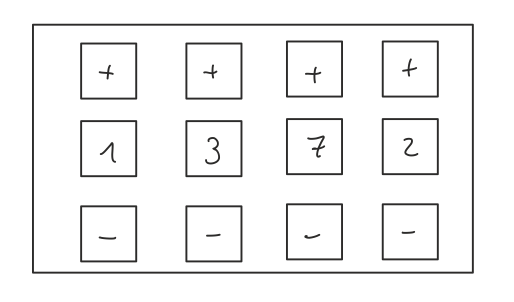
\includegraphics{design1}
\end{minipage}

\begin{minipage}{\linewidth}
  \centering
  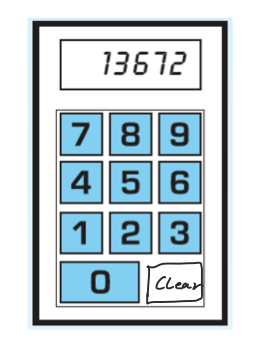
\includegraphics{design2}
\end{minipage}
